
\begin{intro}
  Linear algebra deals with abstract vector spaces, but most results
  on linear mappings are restricted to finite dimensional spaces,
  since they exploit the fact that we can choose a basis of finite
  length. After such a choice, every linear mapping is well-defined by
  assigning its values on the finite set of basis vectors. Thus,
  vector spaces and linear mappings, while typically sets with
  infinitely many elements, can be characterized completely by finite
  sets. The resulting theory yields very strong results by simple means.

  The choice of a basis becomes a more involved endeavor if we allow
  for spaces that do not have a finite basis. We can actually go by
  two very different routes. The route of Hamel bases, which are bases
  of inifintely many vectors, but in order to represent a vector in
  such a basis, we only allow for finite linear combinations.
  
  The other route defines a Schauder basis as a set of vectors, such
  that every vector in the space is the linear combination of
  infinitely many basis vectors. In order to define such a linear
  combination, we have to define the meaning of such an infinite sum,
  namely the convergence of the sum. In the course of such a
  definition, we will learn about a natural extension of
  Euclidean\footnote{We will not distinguish between
    Euclidean real spaces and unitary complex spaces.}
  spaces, namely pre-Hilbert and Hilbert spaces.

  Hilbert spaces share with $\R^n$ the concept of orthogonality. Thus,
  they allow us to define orthogonal bases. Furthermore, they admit
  simple generalizations of the theorem, that for any matrix $A$ with
  $n$ columns there exists an orthogonal decomposition
  \begin{gather}
    \R^n = \ker A \oplus \range{A^T}.
  \end{gather}
\end{intro}

%%%%%%%%%%%%%%%%%%%%%%%%%%%%%%%%%%%%%%%%%%%%%%%%%%%%%%%%%%%%%%%%%%%%%%
%%%%%%%%%%%%%%%%%%%%%%%%%%%%%%%%%%%%%%%%%%%%%%%%%%%%%%%%%%%%%%%%%%%%%%
\section{Banach and Hilbert spaces}
%%%%%%%%%%%%%%%%%%%%%%%%%%%%%%%%%%%%%%%%%%%%%%%%%%%%%%%%%%%%%%%%%%%%%%
%%%%%%%%%%%%%%%%%%%%%%%%%%%%%%%%%%%%%%%%%%%%%%%%%%%%%%%%%%%%%%%%%%%%%%

\begin{Notation}{field-k}
  This section deals with real and complex vector spaces. Therefore,
  if nothing else is noted, the field $\mathbb K$ may be $\R$ or $\C$.
\end{Notation}

\begin{Definition}{functional}
  Let $V$ be a vector space. A \define{functional} on $V$ is a mapping
  $\phi\colon V\to \mathbb K$. A functional is called \define{linear}, if
  there holds
  \begin{gather}
    \label{eq:lafa:3}
    \phi(\alpha v+w) = \alpha \phi(v)+\phi(w),
    \qquad\forall \alpha\in \mathbb K, \;v,w\in V.
  \end{gather}
  A functional $\phi\colon V\to \R^+_0$ is called \define{sublinear}, if
  \begin{subequations}
    \label{eq:lafa:4}    
    \begin{xalignat}2
      \label{eq:lafa:16}
      \phi(\alpha v) &= \abs{\alpha}\phi(v)
      && \forall\alpha\in\mathbb K,\;v\in V,\\
      \label{eq:lafa:17}
      \phi(v+w) &\le \phi(v)+\phi(w)
      && \forall v,w\in V.
    \end{xalignat}
  \end{subequations}
  A functional $\phi\colon V\to \R^+_0$ is called \define{definite}, if
  \begin{gather}
    \label{eq:lafa:5}
    \phi(v)=0 \quad \Rightarrow v=0 \qquad\forall v\in V.
  \end{gather}
  A \define{norm} $\norm\cdot$ on $V$ is a definite, sublinear functional on $V$.
\end{Definition}

\begin{remark}
  The properties of sublinear functionals in
  equation~\eqref{eq:lafa:4} are called
  \define{homogeneity}~\eqref{eq:lafa:16} and
  \define{subadditivity}~\eqref{eq:lafa:17}. The
  inequality~\eqref{eq:lafa:17} is also known as \define{triangle
    inequality}.
\end{remark}

\begin{Definition}{inner-product}
  Let $V$ be a vector space over $\mathbb K$ with $\mathbb K = \mathbb
  C$ or $\mathbb K = \R$. An \define{inner product} on $V$ is a mapping
  $\scal(.,.): V\times V \to \mathbb K$ with the properties
  \begin{xalignat}2
    \label{eq:inner-product:1}
    \scal(\alpha x+y,z) &= \alpha \scal(x,z) + \scal(y,z)
    && \forall x,y,z \in V; \alpha \in \mathbb K\\
    \label{eq:inner-product:2}
    \scal(x,y) &= \overline{\scal(y,x)} && \forall x,y \in V \\
    \label{eq:inner-product:3}
    \scal(x,x) & \ge 0 \quad\forall x\in V &&\text{and} \\
    \label{eq:inner-product:4}
    \scal(x,x) & =0 \Leftrightarrow x=0,
  \end{xalignat}
  usually referred to as (bi-)linearity, symmetry, and
  definiteness. We note that linearity in the second argument follows
  immediately by symmetry.
\end{Definition}

\begin{Theorem*}{bcs-inequality}{Bunyakovsky-Cauchy-Schwarz inequality}
  For every \putindex{inner product} there holds the inequality
  \begin{gather}
    \label{eq:lafa:6}
    \scal(v,w) \le \sqrt{\scal(v,v)} \sqrt{\scal(w,w)}.
  \end{gather}
  Equality holds if and only if $v$ and $w$ are collinear.
\end{Theorem*}

\begin{proof}
  The case $w = 0$ is trivial. Without loss of generality we can therefore
  assume that $w \not = 0$. Define $\lambda \in \C$ as $\lambda =
  \frac{\scal(v,w)}{\scal(w,w)}$. By (\ref{eq:inner-product:3}) we have
  \begin{gather*}
  0 \le \scal(v - \lambda w, v - \lambda w) \label{eq:bcs:1}
  \end{gather*}
  and by ~(\ref{eq:inner-product:2}) the right-hand side extends to
  \begin{gather*}
  \scal(v, v) - \scal(v, \lambda w) - \scal(\lambda w, v) +
    \scal(\lambda w, \lambda w) \\
  = \scal(v, v) - \overline{\lambda} \scal(v, w) - \overline{\lambda} \scal(v, w)
    + \lambda \overline{\lambda}\scal(w, w).
  \end{gather*}
  Evaluating $\lambda$ yields the inequality
  \begin{gather*}
  0 \le \scal(v, v) - \frac{\overline{\scal(v, w)} \scal(v, w)}{\scal(w, w)}
    - \frac{\overline{\scal(v, w)} \scal(v, w)}{\scal(w, w)}
    + \frac{\overline{\scal(v, w)} \scal(v, w)\scal(w, w)}{\scal(w, w)^2}.
  \end{gather*}
  The result follows from multiplication with $\scal(w, w)$ and arranging
  the summands.
  
  For the second part let $v, \, w$ be colinear, i.e. there is a $\lambda \in
  \mathbb K$ such that $v = \lambda w$. Then deducing the equality is trivial.
  Now let equality hold for (\ref{eq:lafa:6}). We immediately get that the equality
  must also hold for
  \begin{gather*}
  0 = \scal(v - \lambda w, v - \lambda w).
  \end{gather*}
  However, by ~(\ref{eq:inner-product:4}) this implies
  \begin{gather*}
  0 = v - \lambda w.
  \end{gather*}
  Thus, $v$ and $w$ are colinear.
\end{proof}

\begin{Lemma}{inner-product-norm}
  Every inner product defines a norm by
  \begin{gather}
    \label{eq:lafa:7}
    \norm{v} = \sqrt{\scal(v,v)}.
  \end{gather}
\end{Lemma}

\begin{proof}
  Definiteness and homogeneity follow from the properties of the inner
  product. It remains to show the triangle inequality
  \begin{gather*}
    \norm{u+v} \le \norm{u}+\norm{v}.
  \end{gather*}
  Squaring the left hand side yields with the
  Bunyakovsky-Cauchy-Schwarz inequality
  \begin{multline*}
    \norm{u+v}^2
    = \scal(u+v,u+v)
    = \norm{u}^2 + 2 \scal(u,v) + \norm{v}^2
    \\
    \le \norm{u}^2 + 2 \norm u \norm v + \norm{v}^2
    = \bigl(\norm u + \norm v\bigr)^2.
  \end{multline*}
\end{proof}

\begin{Lemma}{orthogonal-equations}
  For two vectors $u,v$ in an \putindex{inner product} space holds the
  \putindex{Pythagoras} theorem
  \begin{gather}
    \label{eq:lafa:14}
    \scal(u,v) = 0,
    \quad\Rightarrow\quad
    \norm{u+v}^2 = \norm u^2 +\norm v^2.
  \end{gather}
  Furthermore, there holds the \putindex{parallelogram identity}
  \begin{gather}
    \label{eq:lafa:15}
    \norm{u+v}^2 + \norm{u-v}^2 = 2\norm{u^2}+2\norm{v}^2.
  \end{gather}
\end{Lemma}

\begin{proof}
  The Pythagorean Theorem ~(\ref{eq:lafa:14}) follows directly with
  \begin{gather*}
    \norm{u+v}^2
    = \scal(u+v,u+v)
    = \norm{u}^2 + 2 \scal(u,v) + \norm{v}^2
    = \norm{u}^2 + \norm{v}^2
  \end{gather*}
  Using that $\overline{-1} = -1$ we get that
  \begin{gather*}
  \scal(u+v,u+v) + \scal(u-v,u-v) = 2\norm{u^2} + 2\norm{v}^2.
  \end{gather*}
\end{proof}

\begin{Definition}{complete}
  A space $V$ with is \define{complete} with respect to a norm, if all
  \putindex{Cauchy sequence}s with elements in $V$ have their limit in
  $V$. A subspace $W\subset V$ is \define{closed} if it is complete.

  The \define{completion} of a space $V$ with respect to a norm
  consists of the space $V$ and the limits of all Cauchy sequences in
  $V$.
  
  We denote the completion of a space $V$ by
  \begin{gather}
    \label{eq:lafa:8}
    \overline{V} = \overline{V}^{\norm{\cdot}_V}.
  \end{gather}
\end{Definition}

\begin{remark}
  \slideref{Definition}{complete} is intuitive, but mathematically
  vague, since the limit of a Cauchy sequence is defined by the
  completion process itself. To avoid this we define the limit of a
  Cauchy-sequence as an equivalence class on the space of
  Cauchy-sequences themselves: We call two Cauchy sequences
  $\{v_n\}_{n = 1, \dots}$ and $\{w_n\}_{n = 1, \dots}$ equivalent, if
  \begin{gather*}
    \norm{v_n-w_n} \to 0
    \quad\text{as}\quad
    n\to \infty.
  \end{gather*}
  If the limits of both sequences exist, we know that this condition
  is equivalent to both limits being equal. If the limits do not exist,
  they are defined by these equivalence classes in a way consistent with
  the standard notion of limits.
\end{remark}

\begin{Definition}{Banach-hilbert}
  A vector space $V$ equipped with an inner product $\scal(.,.)$ is called
  an \define{inner product space} or \define{pre-Hilbert space}. A
  \define{Hilbert space} is a pre-Hilbert space which is also \putindex{complete}.

  A \define{normed vector space} is a vector space $V$ with a norm
  $\norm\cdot$. We may also write $\norm{\cdot}_V$ to highlight the
  connection. A normed vector space $V$ which is complete with respect to its norm is
  called a \define{Banach space}.
\end{Definition}

\begin{remark}
The concepts presented in \slideref{Definition}{Banach-hilbert} are related as follows:

\begin{figure}[hp]
\begin{center}
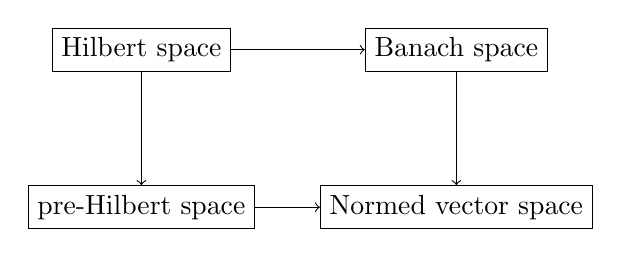
\begin{tikzpicture}[scale=2]
\node[rectangle, draw, fill=white] (N) at (2,0) {Normed vector space};
\node[rectangle, draw, fill=white] (P) at (0,0) {pre-Hilbert space};
\node[rectangle, draw, fill=white] (B) at (2,1) {Banach space};
\node[rectangle, draw, fill=white] (H) at (0,1) {Hilbert space};
\draw[->] (H) -- (B);
\draw[->] (H) -- (P);
\draw[->] (B) -- (N);
\draw[->] (P) -- (N);
\end{tikzpicture}
\end{center}
\end{figure}
\end{remark}

\begin{example}
  For any positive integer, the space $\R^n$ equipped with the
  Euclidean inner product
  \begin{gather*}
    \scal(x,y) = \sum_{i=1}^n x_i y_i
  \end{gather*}
  is a Hilbert space. The same holds for $\mathbb C^n$ and
  \begin{gather*}
    \scal(x,y) = \sum_{i=1}^n x_i \overline{y_i}.
  \end{gather*}
\end{example}

\begin{example}
  The spaces $\ell^2(\R)$ and $\ell^2(\mathbb C)$ of sequences
  $\{x_k\}_{k=1,\dots}$ of real and complex numbers, respectively, are
  Hilbert spaces, if equipped with the inner product
  \begin{gather*}
    \scal(x,y) = \sum_{i=k}^\infty x_k \overline{y_k}
    = \lim_{n\to\infty}\sum_{k=1}^n x_k \overline{y_k}.
  \end{gather*}
  An example for a sequence in $\ell^2(\R)$ is for instance the
  sequence $v = \{1/k\}_{k=1,\dots}$, since
  \begin{gather*}
    \norm{v}^2 = \sum_{k=1}^\infty \frac1{k^2} < \infty.
  \end{gather*}
  The sequence $w = \{1\}_{k=1,\dots}$ is not, since it does not converge
  quadratically.
\end{example}

\begin{Problem}{l2-Cauchy}
  Show that the sequence of sequences defined by
  \begin{gather*}
    v_n = \left\{1,\tfrac12,\dots,\tfrac1n,0,\dots,0\right\},
  \end{gather*}
  is a Cauchy sequence in $\ell^2$.
\end{Problem}

\begin{example}
  On the space of continuous functions on the interval
  $[-\pi/2,\pi/2]$ define the inner product
  \begin{gather*}
    \scal(f,g) = \int_{-\pi/2}^{\pi/2} f(x)g(x)\,dx.
  \end{gather*}
  Let
  \begin{gather*}
    V = \bigl\{f\in C[-\pi/2,\pi/2] \big| \scal(f,f) < \infty \bigr\}.
  \end{gather*}
  Then $V$ is a vector space with an inner product and thus a
  pre-Hilbert space, but it is not a Hilbert space, since for any $n$
  the sum
  \begin{gather*}
    f_n(x) = \frac4\pi \sum_{k=1}^n \frac{\sin\bigl((2k-1) x\bigr)}{2k-1}
  \end{gather*}
  is continuous, but
  \begin{gather*}
    \lim_{n\to\infty} f_n =
    \begin{cases}
      -1 & x<0 \\
      0 & x=0 \\
      1 & x>0
    \end{cases}
  \end{gather*}
  is not.
\end{example}

\begin{Definition}{separable}
  A subset $M$ of a Hilbert space $V$ is called \define{dense}, if
  every vector in $V$ is an accumulation point of $M$, that is, $V$ is
  the closure of $M$.  A Hilbert space is called \define{separable},
  if it has a countable dense subset.
\end{Definition}

\begin{todo}
\begin{remark}
  From the point of view of numerical analysis and computation, spaces
  which are not separable are of limited interest. In fact, every
  result of a numerical calculation is in a finite set. When we look
  at convergence for $n\to\infty$ or $h\to 0$, we are usually studying
  sequences with countable index sets. Therefore, vectors in
  nonseparable spaces cannot be approximated reliably.

  Apart from this remark, it is a goal of these notes to develop a
  framework for applied mathematics without recourse to the axiom of
  choice. Separable spaces allow us for instance to construct bases
  instead of deducing their existence indirectly.
\end{remark}
  I think this remark should be at the beginning of this chapter since
  here the idea behind these notes becomes clearer (to me). Also here,
  it some kind of disturbs the flow of the notes. Perhaps, if it is
  \emph{very} important to you, you could write a review at the end of
  the chapter stating the results and how your goals have been
  accomplished -- and maybe also \emph{why} this goal is so important.
\end{todo}

\begin{Definition}{schauder-basis}
  Let $V$ be a Hilbert space over a field $\mathbb K$. A
  \define{Schauder basis} or short \define{basis} of $V$ is a set
  $\{x_i\}$ of linearly independent vectors with coefficients $i$
  from an index set $I$, such that each $v\in V$ has a representation
  of the form
  \begin{gather*}
    v = \sum_{i\in I} \alpha_i x_i,
  \end{gather*}
  with coefficients $\alpha_i \in \mathbb K$. The index set $I$ may be
  finite in the case of a finite dimensional vector space, or
  countable if $V$ is infinite dimensional and separable. In the
  latter case it is required that the sum in the linear combination
  exists as the limit of a series. In particular, the sum must be a
  Cauchy-sequence with respect to the norm of $V$.
\end{Definition}

\begin{remark}
  In the infinite dimensional case, the norm of the vector space is
  part of the definition of the basis. This is the usual view in
  functional analysis, but it fails if no norm is defined on a general
  vector space $V$. In that case, only finite sums can be admitted,
  leading to a \define{Hamel basis}. While these seem to be more
  immediate extensions of bases on finite dimensional spaces, we will
  not have good use for them here.

  We will use the concept of orthogonality below to establish a
  general existence result for Schauder bases in Hilbert spaces.
\end{remark}

\begin{notation}
  We will use the term \putindex{sequence} to denote an at most
  countable set. The elements of a sequence are numbered by indices
  and the index set is $\mathbb N$ or a subset thereof.
\end{notation}

%%%%%%%%%%%%%%%%%%%%%%%%%%%%%%%%%%%%%%%%%%%%%%%%%%%%%%%%%%%%%%%%%%%%%%
%%%%%%%%%%%%%%%%%%%%%%%%%%%%%%%%%%%%%%%%%%%%%%%%%%%%%%%%%%%%%%%%%%%%%%
\section{Orthogonality}
%%%%%%%%%%%%%%%%%%%%%%%%%%%%%%%%%%%%%%%%%%%%%%%%%%%%%%%%%%%%%%%%%%%%%%
%%%%%%%%%%%%%%%%%%%%%%%%%%%%%%%%%%%%%%%%%%%%%%%%%%%%%%%%%%%%%%%%%%%%%%

\begin{Definition}{orthogonal}
  Let $V$ be an inner product space over a field $\mathbb K$. Two
  vectors $x,y\in V$ are called \define{orthogonal} if $\scal(x,y) = 0$. We
  write $x\perp y$. Let $W$ be a subspace of $V$. We say that a vector $v$
  is orthogonal to the subspace $W$, if it is orthogonal to every vector in
  $W$.

  A set of nonzero mutually orthogonal vectors
  $\{x_i\} \subset V$ is called \define{orthogonal set}. If
  additionally $\norm{x_i} = 1$ for all vectors, it is called an
  \define{orthonormal set}. These notions transfer directly from
  finite to countable sets.
\end{Definition}

\begin{Definition}{orthogonal-complement}
  Let $W\subset V$ be a subspace of a Hilbert space $V$. We define its
  \define{orthogonal complement} $\ortho W\subset V$ by
  \begin{gather}
    \label{eq:infsup:7}
    \ortho W = \bigl\{v\in V \big| \scal(v,w)_{V} = 0
    \;\forall\,w\in W\bigr\}.
  \end{gather}
\end{Definition}

\begin{Lemma}{orthogonal-closed}
  The orthogonal complement $\ortho W$ of a subspace $W\subset V$
  is closed in the sense of ~\slideref{Definition}{complete}.
\end{Lemma}

\begin{proof}
  By the \putindex{Bunyakovsky-Cauchy-Schwarz inequality}, the inner
  product is continuous on $V\times V$. Therefore, the mapping
  \begin{align*}
    \phi_w\colon V &\to \R,\\
    v&\mapsto \scal(v,w),
  \end{align*}
  is continuous. For any $w\in W$, the kernel of $\phi_w$ is closed as
  the pre-image of the closed set $\{0\}$. Since
  \begin{gather*}
    \ortho W = \bigcap_{w\in W} \ker{\phi_w},
  \end{gather*}
  it is closed as the intersection of closed sets.
\end{proof}

\begin{Theorem}{orthogonal-complement}
  Let $W$ be a subspace of a Hilbert space $V$ and $W^\perp$ its
  orthogonal complement. Then, $W^\perp = \overline{W}^\perp$. Further,
  $V = W \oplus W^\perp$ if and only if $W$ is closed.
\end{Theorem}

\begin{proof}
  Clearly, $\overline{W}^\perp \subset W^\perp$ since
  $W\subset\overline{W}$. Let now $u\in W^\perp$. Then, $\phi =
  \scal(u,\cdot)$ is a continuous linear functional on $V$. Therefore,
  if a sequence $w_n \subset W$ converges to $w\in \overline{W}$, we
  have
  \begin{gather*}
    \scal(u,w) = \lim_{n\to\infty} \scal(u,w_n) = 0,
  \end{gather*}
  since $u \in W^\perp$. Hence, $u\in \overline{W}^\perp$ and
  $W^\perp = \overline{W}^\perp$.

  Now, the ``only if'' follows by the fact, that if $W$ is not
  closed, there is an element $w\in \overline{W}$ but not in $W$ such that
  $\scal(w,u)=0$ for all $u\in W^\perp$. Thus, $w\not\in W^\perp$ and
  consequently $w\not\in W^\perp \oplus W$.

  Let now $W$ be closed. We show that for all $v \in V$ there is a unique
  decomposition
  \begin{gather}
    \label{eq:infsup:8}
    v = w + u,\qquad \text{with} \qquad w\in W, \;u\in W^\perp.
  \end{gather}
  This is equivalent to $V = W \oplus W^\perp$. Uniqueness follows,
  since
  \begin{gather*}
    v = w_1+u_1 = w_2+u_2
  \end{gather*}
  implies that for any $y\in V$
  \begin{gather*}
    0 = \scal(w_1-w_2+u_1-u_2,y) = \scal(w_1-w_2,y) + \scal(u_1-u_2,y).
  \end{gather*}
  Choosing $y=u_1-u_2$ and $w_1-w_2$ in turns, we see that one of the
  inner products vanishes for orthogonality and the other implies that
  the difference is zero.

  If $v\in W$, we choose $w=v$ and $u=0$. For $v\not\in W$, we prove
  existence by considering that due to the closedness of $W$ there holds
  \begin{gather*}
    d=\inf_{w' \in W} \norm{v-w'} >0.
  \end{gather*}
  Let $w_n$ be a minimizing sequence. Using the parallelogram identity
  \begin{gather*}
    \norm{a+b}^2+\norm{a-b}^2 = 2\norm{a}^2+2\norm{b}^2,
  \end{gather*}
  we prove that $\{w_n\}$ is a Cauchy sequence by
  \begin{align*}
    \norm{w_m-w_n}^2 &= \norm{(v-w_n)-(v-w_m)}^2\\
    &= 2\norm{v-w_n}^2+2\norm{v-w_m}^2-\norm{2v-w_m-w_n}^2\\
    &= 2\norm{v-w_n}^2+2\norm{v-w_m}^2-4\norm*{v-\frac{w_m+w_n}2}^2\\
    &\le 2\norm{v-w_n}^2+2\norm{v-w_m}^2-4d^2,
  \end{align*}
  since $(w_m+w_n)/2\in W$ and $d$ is the infimum. Now we use the
  minimizing property to obtain
  \begin{gather*}
    \lim_{m,n\to\infty}\norm{w_m-w_n}^2 = 2d^2+2d^2 -4d^2=0.
  \end{gather*}
  Since $V$ is given as a Hilbert space and as such complete, $w=\lim w_n$
  exists and by the closedness of $W$, we have $w\in W$. Let $u=v-w$.
  By continuity of the norm, we have $\norm{u}=d$. It remains to show
  that $u\in W^\perp$. To this end, we introduce the variation
  $w+\epsilon \tilde w$ with $\tilde w \in W$ to obtain
  \begin{align*}
    d^2 &\le \norm{v-w-\epsilon \tilde w}^2\\
    &= \norm{u}^2-2\epsilon\scal(u,\tilde w)+\epsilon^2 \norm{\tilde w},
  \end{align*}
  implying for any $\epsilon>0$
  \begin{gather*}
    0\le-2\epsilon\scal(u,\tilde w)+\epsilon^2 \norm{\tilde w},
  \end{gather*}
  which requires $\scal(u,\tilde w) = 0$. Since $\tilde w \in W$ was chosen
  arbitrarily, we have $u \in W^\perp$.
\end{proof}

\begin{Corollary}{ortho-density}
  A subspace $W$ of a Hilbert space $V$ is dense in $V$ if and only if
  $\ortho W = \{0\}$.
\end{Corollary}

\begin{proof}
  The ``only if'' is an immediate application of
  \slideref{Theorem}{orthogonal-complement}. For the opposite
  direction, assume $\overline W \neq V$. Choose $v\in V$ such that
  $v\not\in \overline W$. By
  \slideref{Theorem}{orthogonal-complement}, there are unique elements
  $w\in W$ and $u\in \ortho W$, such that $v=w+u$. In particular,
  $u\neq 0$.
  \begin{todo}
    Make this a lemma about  the fact that on the polar space!!
    Now, let $\phi = \scal(u,.) \in V^*$. Then, there holds
    \begin{align*}
      \phi(u) &= \norm{u}_V^2 \neq 0 \\
      \phi(w) &= 0 \quad\forall w\in W.
    \end{align*}
    Thus, from the fact that $W$ is not dense follows the existence of a
    linear functional which vanishes on $W$, but not on $V$.
  \end{todo}
\end{proof}

\begin{Definition}{ortho-projection}
  Let $W$ be a closed subspace of the Hilbert space $V$ and $\ortho W$
  be its orthogonal complement. Then, the
  \define{orthogonal projection} operators
  \begin{gather}
    \label{eq:lafa:9}
    \begin{split}
      \Pi_W &\colon V\to W\\
      \Pi_{\ortho W} &\colon V\to \ortho W\\
    \end{split}
  \end{gather}
  are defined by the unique decomposition
  \begin{gather}
    \label{eq:lafa:10}
    v = \Pi_W v + \Pi_{\ortho W} v.
  \end{gather}
\end{Definition}

\begin{Lemma*}{gram-schmidt}{Gram--Schmidt}
  For every linearly independent sequence of
  vectors $\{v_i\}$ there is an up to scaling unique orthonormal set
  $\{x_i\}$ with the property that
  \begin{gather*}
    \forall n\in \mathbb N:\quad
    \operatorname*{span}_{i=1,\dots,n} \{x_i\}
    =
    \operatorname*{span}_{i=1,\dots,n} \{v_i\}.
  \end{gather*}
\end{Lemma*}

\begin{proof}
  The proof uses induction over the length of the sequence.  Beginning
  with $v_1$, choose $x_1 = v_1$, which is nonzero by the assumption
  of linear independence.

  Assume now that the lemma holds for the elements $v_1,\dots,v_k$, such that
  \begin{gather*}
    V_k = \spann{v_1,\dots,v_k} = \spann{x_1,\dots,x_k}.
  \end{gather*}
  Again, by linear independence, $v_{k+1}$ is not in $V_k$ and $V_k$
  is closed since it is finite dimensional. Hence, we can choose
  \begin{gather*}
    \tilde x_{k+1} = \Pi_{\ortho V_k} v_{k+1},
    \qquad \frac{\tilde x_k}{\norm{\tilde x_k}}.
  \end{gather*}
\end{proof}

  
\begin{Theorem}{Hilbert-basis}
  Every separable Hilbert space has an at most countable, orthonormal
  Schauder basis.
\end{Theorem}

% See e.g.~\cite{Yosida80}.
\begin{proof}
  First, let $M$ be a countable dense subset
  of $V$, which exists due to the separability assumption. Now choose
  any numbering of $M$ and $v_1$ the first nonzero element in
  $M$. For $i=2,\dots,\infty$ choose with $v_1,\dots,v_{i-1}$ given
  $v_i$ as the next vector in $M$ which is not in the subspace spanned
  by $v_1,\dots,v_{i-1}$. This procedure generates an at most
  countable sequence $\{v_1, \dots, v_i\}_{i=1, \dots}$ of linearly
  independent vectors. It will only stop, if $V$ is finite dimensional.
  Furthermore, we have that every element in $M$ can be written as a finite
  linear combination of these vectors: Assume $w \in M$ as $w \not \in
  \spann{v_1,\dots,v_k}$ for any natural number $k$. Since $M$ is countable,
  we will eventually get to $w$ which then --- by definition of the sequence
  --- will be added to it as $v_{k+1} = w$.
  
  The sequence $\{v_i\}_{i=1,\dots}$ is a Schauder basis for $V$. In fact, given a
  vector $v\in V$ we have to show that for every $\epsilon$, there is
  a finite linear combination $s_n = \sum_{i=1}^n \alpha_i v_i$ such
  that $\norm{v-s_n} < \epsilon$. Let by separability $w_\epsilon$ be in
  $M$ such that $\norm{v-w_\epsilon} < \epsilon$. Since
  $w_\epsilon in M$, there is $n$ such that $s_n = w_\epsilon$.

  Finally, we use the Gram--Schmidt procedure to orthogonalize the
  sequence.
\end{proof}

\begin{Theorem}{Hilbert-basis-completion}
  Let $W$ be a closed subspace of a separable Hilbert space $V$ and
  $\{x_k\}$ be an orthonormal basis for $W$. Then, this basis can be
completed to be a basis of $V$.
\end{Theorem}

\begin{Problem}{Schauder-basis-completion}
  Prove \slideref{Theorem}{Hilbert-basis-completion}. Take into account
  that $W$ is not assumed finite dimensional.
\end{Problem}

\begin{example}
  In the Hilbert spaces $\R^n$, $\mathbb C^n$, $\ell^2(\R)$, and
  $\ell^2(\mathbb C)$, an orthonormal basis is obtained by choosing
  basis vectors $x_i$ with entries $x_{i,j} = \delta_{ij}$.
\end{example}

\begin{Lemma*}{Bessel-inequality}{Bessel inequality}
  Let $\{x_i\}$ be an orthonormal basis of the Hilbert space $V$. For
  $v\in V$, define %the \define{Fourier coefficient}s
  \begin{gather}
    \label{eq:lafa:18}
    \alpha_i = \scal(v,x_i), \qquad i=1,\dots
  \end{gather}
  Then,
  \begin{gather}
    \label{eq:lafa:18a}
    \sum_{i=1}^\infty \abs{\alpha_i}^2 \le \norm{v}_V^2.
  \end{gather}
\end{Lemma*}

\begin{proof}
  For $n\in \mathbb N$, we have
  \begin{align*}
    \norm*{v-\sum_{i=1}^n \alpha_i x_i}^2
    &= \scal(v-\sum \alpha_i x_i,v-\sum \alpha_i x_i) \\
    &= \norm{v}^2 -\scal(v,\sum \alpha_i x_i)
      -\scal(\sum \alpha_i x_i, v) + \sum \abs{\alpha_i}^2\\
    &= \norm{v}^2 - \sum \abs{\alpha_i}^2.
  \end{align*}
  Since the left hand side is nonnegative, the Bessel inequality holds.
\end{proof}

\begin{Lemma*}{Parseval-identity}{Parseval identity}
  Under the same assumptions as in \slideref{Lemma}{Bessel-inequality}
  the sequence
  \begin{gather*}
    f_n = \sum_{i=1}^n \alpha_i x_i = \sum_{i=1}^n \scal(f, x_i) x_i
  \end{gather*}
  converges to $f$ in $V$ and there holds
  \begin{gather}
    \label{eq:lafa:19}
    \norm{f}^2 = \sum_{i=1}^\infty \abs{\alpha_i}^2.
  \end{gather}
\end{Lemma*}

\begin{proof}   
  First, we will show that the series $\{f_n\}_{n=1,\dots}$ is a
  Cauchy sequence and, using the completeness of $V$, deduce that
  $\{f_n\}_{n=1,\dots}$ does indeed converge in $V$. Second, we will
  prove that indeed there holds $f_n \to f$ as $n \to \infty$.
  Finally, it is easy to show that $\norm{f}^2$ does indeed equal to
  $\sum_{i=1}^\infty \abs{\scal(f, x_i)}^2$.
  
  Take $m,\, n \in \mathbb{N}$ with $n>m$ and consider
  \begin{gather*}
    \norm{f_n - f_m}^2 = \norm{\sum_{i=m+1}^n \scal(f, x_i) x_i}^2.
  \end{gather*}
  Since $\{x_i\}_{i=1,\dots}$ are indeed pairwise orthogonal, we can
  use the Pythagorean Theorem to obtain that the above equation becomes
  \begin{gather*}
    \sum_{i=m+1}^n \norm{\scal(f, x_i) x_i}^2
      = \sum_{i=m+1}^n \abs{\scal(f, x_i)}^2  \norm{x_i}^2.
  \end{gather*}
  Furthermore, the $\{x_i\}_{i=1,\dots}$ are orthonormal. Hence,
  $\norm{x_i} = 1$ for all $i=1, \dots$. The above equation simplifies to
  \begin{gather*}
    \sum_{i=m+1}^n \abs{\scal(f, x_i)}^2.
  \end{gather*}
  By Bessel's inequality we know that
  \begin{gather*}
    \sum_{i=1}^\infty \abs{\scal(f, x_i)}^2 \le \norm{f}_V^2
  \end{gather*}
  and hence $\{f_n\}_{n=1,\dots}$ converges. Therefore, the difference
  $\norm{f_n - f_m}^2$ can be arbitrarily small and hence the sequence
  $\{f_n\}_{n=1,\dots}$ is Cauchy. Since $V$ is given as a Hilbert space,
  $V$ is also complete. By that, the sequence $\{f_n\}_{n=1,\dots}$
  converges to some $\bar{f} \in V$.
  
  To prove that $f = \bar{f}$, consider $\scal(f-\bar{f}, x_k)$ for some
  $k \in \mathbb{N}$. If we show that this equals zero, we know that
  $(f-\bar{f}) \perp x_k$ for any $k \in \mathbb{N}$. 
  By linearity of the inner product, we have that
  \begin{align*}
  \scal(f-\bar{f}, x_k) &= \scal(f, x_k)
    -\sum_{i=1}^\infty \scal(f, x_i)\scal(x_i, x_k) \\
    &= \scal(f, x_k) - \scal(f, x_k) = 0.
  \end{align*}
  Here we used that $\scal(x_i, x_k) = \delta_{i,k}$. Hence $(f-\bar{f})
  \perp x_k$. Since $\{x_k\}_{k=1,\dots}$ form a basis, there holds
  \begin{gather}
  \label{eq:lafa:18b}
  f = \bar{f} = \lim_{n\to \infty} \sum_{i=1}^n \scal(f, x_i) x_i.
  \end{gather}
  
  Finally, we have that
  \begin{gather*}
    \norm{f} = \norm{\lim_{n\to \infty} \sum_{i=1}^n \scal(f, x_i) x_i}.
  \end{gather*}
  By continuity of the norm and equation ~(\ref{eq:lafa:18b}) the above
  equation becomes
  \begin{gather*}
    \lim_{n\to \infty} \norm{\sum_{i=1}^n \scal(f, x_i) x_i}.
  \end{gather*}
  Using the Pythagorean theorem and the orthogornality we obtain
  \begin{gather*}
  \lim_{n\to \infty} \sum_{i=1}^n \abs{\scal(f, x_i)} \cdot 1
    = \sum_{i=1}^\infty \abs{\scal(f, x_i)}.
  \end{gather*}
  Thus, Parseval's identity has been established as desired.
\end{proof}

\begin{remark}
  In his monograph ``Mémoire sur les séries et sur l'intégration complète
  d'une équation aux différences partielles linéaires du second ordre,
  à coefficients constants'' from April 5, 1799, Marc-Antoine Parseval
  published his ``original'' identity for Fourier coefficients. The other
  ingredients for more more generalized formulation took some more time:
  In 1898, Guiseppe Peano came up with the theory of pre-Hilbert spaces,
  or, at that time, inner product spaces. In 1907, Riesz and Fischer
  (independently) came up with their famous theorem, the completeness of
  $L^p$ for $0<p \le \infty$ which has been used for $p=2$. The more
  general version of his theorem was published in Titchmarchs book in
  1939. In the meantime, someone must have connected the dots and found
  this more general formulation. Unfortunately, his/her name has apparently
  been forgotten.
\end{remark}

%%%%%%%%%%%%%%%%%%%%%%%%%%%%%%%%%%%%%%%%%%%%%%%%%%%%%%%%%%%%%%%%%%%%%%
%%%%%%%%%%%%%%%%%%%%%%%%%%%%%%%%%%%%%%%%%%%%%%%%%%%%%%%%%%%%%%%%%%%%%%
\section{Linear operators}
%%%%%%%%%%%%%%%%%%%%%%%%%%%%%%%%%%%%%%%%%%%%%%%%%%%%%%%%%%%%%%%%%%%%%%
%%%%%%%%%%%%%%%%%%%%%%%%%%%%%%%%%%%%%%%%%%%%%%%%%%%%%%%%%%%%%%%%%%%%%%

\begin{intro}
  Linear mappings are the next central topic of linear algebra, which
  we want to extend to infinite dimensional spaces. Here, the basic
  definition remains the same, that is, a \define{linear operator} is
  a mapping of a Hilbert space $V$ to a Hilbert space $W$ which is
  compatible with vector operations. But Hilbert spaces have
  additional structure by their norms and their completeness.
\end{intro}

\begin{Definition}{linear-operator}
  Let $V,W$ be two vector spaces. A \define{linear mapping} or
  \define{linear operator} $L\colon V\to W$ is a mapping such that
  \begin{gather*}
    L(\alpha u+\beta v) = \alpha L(u) + \beta L(v),
  \end{gather*}
  for all $\alpha,\beta\in\mathbb K$ and for all $u,v\in V$.
%  such that  $L(u)$ and $L(v)$ are defined.
\end{Definition}

\begin{Definition}{bounded-operator}
  A linear operator $L\colon V\to W$ is called \define{bounded} on $V$
  if there exists a constant $c$ such that
  \begin{gather}
    \label{eq:lafa:11}
    \norm{L v}_W \le c \norm{v}_V
    \quad\forall v\in V.
  \end{gather}
  We define the operator norm $\norm{L}$ as
  \begin{gather}
    \label{eq:lafa:12}
    \norm L = \sup_{v\in V} \frac{\norm{L v}_W}{\norm{v}_V}.
  \end{gather}
\end{Definition}

\begin{remark}
  Every linear mapping of a finite dimensional space is continuous,
  even \putindex{Lipschitz continuous}. This follows easily from the
  matrix representation. The fact that a linear mapping can be
  unbounded is a new property of infinite dimensional spaces, which
  will be discussed in §\ref{???}.
\end{remark}

\begin{Theorem}{continuous-operator}
  A linear operator $L\colon V\to W$ is continuous on $V$ if and only
  if it is bounded. It is continuous everywhere if it is continuous in
  a single point.
\end{Theorem}

\begin{todo}
\begin{proof}
  Let $L\colon V\to W$ be bounded with boundary constant $c$ and let
  the sequence $\{v_n\}_{n=1,\dots} \subset V$ converge to some 
  $v \in V$ as $n \to \infty$. Using the boundedness of $L$, we obtain
  \begin{gather*}
    \norm{Lv_n - Lv} = \norm{L(v_n - v)} \le c\norm{v_n - v}.
  \end{gather*}
  By the convergence of $\{v_n\}_{n=1,\dots}$ we get that $Lv_n \to Lv$
  as $n \to \infty$. Hence, $L$ is continous.
  
  Now assume $L$ as unbounded. Then, there exists a sequence
  $\{v_n\}_{n=1,\dots}$ such that $\norm{Lv_n}$ diverges as $n \to \infty$.
  Define the sequence $\{\tilde{v}_n\}_{n=1,\dots}$ as
  \begin{gather*}
    \tilde{v}_n = \frac{v_n}{\norm{Lv_n}}.
  \end{gather*}
  We immediately get that $\norm{L\tilde{v}_n} = 1$ for all $n$, but
  $\norm{\lim_{n\to\infty}L\tilde{v}_n} = 0$. Thus, $L$ is not continous.
  
  For the second equivalence note that continuity trvially implies
  continuity in a single point, e.g. $x \in V$. Now let $L$ be continous 
  n $x$ and take the sequence $\{v_n\}_{n=1,\dots} \subsbet V$ converging
  to $v \in V$ Then, $\{v_n-(v-x)\}_{n=1,\dots}$ converges to $x$ and by
  continuity we have $L(v_n-(v-x)) = Lv_n - Lv + Lx \to Lx$ as $n \to \infty$.
  This yields $Lv_n \to Lv$ and thus, $L$ is continous.
\end{proof}
\end{todo}

%%%%%%%%%%%%%%%%%%%%%%%%%%%%%%%%%%%%%%%%%%%%%%%%%%%%%%%%%%%%%%%%%%%%%%
%%%%%%%%%%%%%%%%%%%%%%%%%%%%%%%%%%%%%%%%%%%%%%%%%%%%%%%%%%%%%%%%%%%%%%
\section{The dual space}
%%%%%%%%%%%%%%%%%%%%%%%%%%%%%%%%%%%%%%%%%%%%%%%%%%%%%%%%%%%%%%%%%%%%%%
%%%%%%%%%%%%%%%%%%%%%%%%%%%%%%%%%%%%%%%%%%%%%%%%%%%%%%%%%%%%%%%%%%%%%%

\begin{Definition}{dual-space}
  A \define{linear functional} on a vector space $V$ is a
  \putindex{linear mapping} from $V$ to $\mathbb K$.

  The \define{dual space} $V^*$ of a vector space $V$, also called the
  \define{normed dual}, is the space of all bounded linear functionals
  on $V$ equipped with the norm
  \begin{gather}
    \norm{\phi}_{V^*} = \sup_{v\in V} \frac{\phi(v)}{\norm{v}_V}.
  \end{gather}
\end{Definition}

\begin{intro}
  From linear algebra, we know that the dual of $\R^n$ is $\R^n$
  itself, and for every basis $\{e_1,\dots,e_n\}$ we can define a dual
  basis $\{d_1,\dots,d_n\}$ by the conditions
  \begin{gather*}
    d_i(e_j) = \delta_{ij}.
  \end{gather*}
  The following results establish similar results for general Hilbert
  spaces.
\end{intro}

\begin{Theorem*}{Riesz-representation}{Riesz representation theorem}
  Let $V$ be a Hilbert space. Then, $V$ is isometrically isomorphic to
  $V^*$. In particular, there is an isomorphism
  \begin{gather}
    \label{eq:lafa:1}
    \begin{split}
      \varrho\colon V & \to V^*, \\
      y & \mapsto f,
    \end{split}
  \end{gather}
  such that
  \begin{gather}
    \label{eq:lafa:2}
    \begin{split}
    \scal(x,y) &= f(x) \qquad \forall x\in V,\\
    \norm{y}_V &= \norm{f}_{V^*}.
    \end{split}
  \end{gather}
  We refer to $\varrho$ as \define{Riesz isomorphism}.
\end{Theorem*}

% from Yosida III.6
\begin{proof}
  The proof is constructive and makes use of the orthogonal
  complement.

  First, it is clear that for any $y\in V$ a linear functional
  $f\in V^*$ is defined by $f(\cdot) = \scal(y,\cdot)$. Furthermore,
  $\varrho$ is injective, since
  \begin{gather*}
    \scal(x,y) = 0 \qquad\forall x\in V
  \end{gather*}
  implies $y\in \ortho V = \{0\}$. By the
  \putindex{Bunyakovsky-Cauchy-Schwarz inequality}, we have
  \begin{gather*}
    \norm{f}_{V^*} = \sup_{x\in V}\frac{\abs{f(x)}}{\norm{x}_V}
    = \sup_{x\in V}\frac{\abs{\scal(x,y)}}{\norm{x}_V}
      \le \norm{y}_V,
  \end{gather*}
  with equality for $x=y$.  It remains to show that $\varrho$ is
  surjective. To this end, let $f\in V^*$ be arbitrary and let
  $N = \ker f$. If $N=V$, we choose $y=0$. If not, choose
  $\ortho y \in \ortho N$ and let
  \begin{gather}
    \label{eq:lafa:13}
    y = \frac{\overline{f(\ortho y)}}{\norm*{\ortho y}^2} \ortho y \in
    \ortho N,
  \end{gather}
  such that $f(y) = \abs*{f(\ortho y)}^2/\norm*{\ortho y}^2 \neq 0$.
  Let now $x\in V$ be chosen arbitrarily. Then, there holds
  \begin{gather*}
    x = \left(x-\frac{f(x)}{f(y)} y\right)
    + \frac{f(x)}{f(y)} y.
    \\
  \end{gather*}
  Since
  \begin{gather*}
      f = \left(x-\frac{f(x)}{f(y)} y\right) 
      = \left(f(x)-f(x) \frac{f(y)}{f(y)}\right)
      = 0,
  \end{gather*}
  this decomposition amounts to $x = x^0+\ortho x$ with $x^0\in N$ and
  $\ortho x \in \ortho N$. It is unique according to
  \slideref{Definition}{ortho-projection}. Thus, we have that $\ortho x$ is a
  multiple of $y$, say $\ortho x=\alpha y$ and thus
  \begin{gather*}
    \begin{aligned}
    f(x) &= f(x^0) + f(\ortho x)
    &=& \alpha f(y)
    &=& \alpha \frac{\abs*{f(\ortho y)}^2}{\norm*{\ortho y}^2}
    \\
    \scal(x,y) &= \scal(x^0,y)  + \scal(\ortho x,y)
    &=& \alpha \norm{y}_V^2
    &=& \alpha \frac{\abs*{f(\ortho y)}^2}{\norm*{\ortho y}^4}
    \norm*{\ortho y}^2
    \end{aligned}
  \end{gather*}
  Hence, the two terms are equal and $\varrho$ is surjective.
\end{proof}

%%%%%%%%%%%%%%%%%%%%%%%%%%%%%%%%%%%%%%%%%%%%%%%%%%%%%%%%%%%%%%%%%%%%%%
%%%%%%%%%%%%%%%%%%%%%%%%%%%%%%%%%%%%%%%%%%%%%%%%%%%%%%%%%%%%%%%%%%%%%%
\section{Weak convergence and compact operators}

\begin{example}
  Let $\phi:\ell^2(\R)\to\ell^2(\R)$ be such that
  \begin{gather*}
    v =
    \begin{pmatrix}
      x_1 \\ x_2 \\ \vdots \\ x_k \\ \vdots
    \end{pmatrix}
    \mapsto \phi(v) =
    \begin{pmatrix}
      x_1 \\ 4x_2 \\ \vdots \\ k^2x_k \\ \vdots
    \end{pmatrix}.
  \end{gather*}
  Clearly, $\phi$ is linear. But if we consider the sequence of
  vectors $v_n = \{\delta_{nk}\}$, we see that $v_n \mapsto n^2 v_n$ and
  thus, while the sequence is bounded in $\ell^2(\R)$, its image is
  not.
  
  Moreover, take now the sequence of sequences
  \begin{gather*}
    v_n = \left\{1,\tfrac12,\dots,\tfrac1n,0,\dots,0\right\}
    \quad \mapsto \quad \phi(v_n) = \{1,2,\dots,n,0,\dots,0\}.
  \end{gather*}
  The sequence $v_n$ converges to a limit $v \in \ell^2(\R)$, while
  the sequence $\phi(v_n)$ diverges. While $\phi(v_n)$ is defined for
  all $v_n$, it is not bounded for the limit $v$.
\end{example}

\begin{remark}
  By virtue of completeness of the space, whenever a linear operator
  is not bounded, it must be undefined for some vectors. We could
  exclude such operators from our considerations, but we would
  severely limit the theory we want to develop. Instead, we will
  accept the fact, that we have to extend the notion of a linear
  mapping $\phi: V\to W$ to a linear operator $\phi: V\to W$, which
  may not be defined on all of $V$. The following definition fixes
  this problem somewhat.
\end{remark}

\begin{Definition}{operator-domain}
  Let $\phi: V\to W$ be a linear operator. Then, the \define{domain}
  of $\phi$ is
  \begin{gather*}
    \mathcal D(\phi) = \bigl\{ v\in V \big|
    \phi(v) \in W \bigr\}.
  \end{gather*}
  Here, $\phi(v) \in W$ implies that $\phi(v)$ is also well defined.
\end{Definition}

%%%%%%%%%%%%%%%%%%%%%%%%%%%%%%%%%%%%%%%%%%%%%%%%%%%%%%%%%%%%%%%%%%%%%%
%%%%%%%%%%%%%%%%%%%%%%%%%%%%%%%%%%%%%%%%%%%%%%%%%%%%%%%%%%%%%%%%%%%%%%
\section{Unbounded linear operators}


%%% Local Variables: 
%%% mode: latex
%%% TeX-master: "main"
%%% End: 
